% FlashAttention-2 in Triton (CVPR author-kit layout).
% Build: tectonic main.tex

\documentclass[10pt,twocolumn,letterpaper]{article}

\usepackage[pagenumbers]{cvpr}

% The template's times package only takes effect under pdfLaTeX. Under XeTeX
% (Tectonic) set the Times-compatible TeX Gyre Termes explicitly; math stays in
% Computer Modern, as in the pdfLaTeX build of the template.
\usepackage{fontspec}
\setmainfont{texgyretermes}[
  Extension=.otf, UprightFont=*-regular, BoldFont=*-bold,
  ItalicFont=*-italic, BoldItalicFont=*-bolditalic]
\setmonofont{lmmono10-regular}[Extension=.otf]

\usepackage{algorithm}
\usepackage{algpseudocode}
\usepackage{tikz}
\usetikzlibrary{positioning,arrows.meta,fit}
\usepackage{multirow}

\definecolor{cvprblue}{rgb}{0.21,0.49,0.74}
\usepackage[pagebackref,breaklinks,colorlinks,allcolors=cvprblue]{hyperref}

\def\confName{CVPR}
\def\confYear{2027}

\newcommand{\lse}{\widehat{\mathrm{lse}}}
\newcommand{\TF}{\,TFLOP/s}
\algrenewcommand\algorithmiccomment[1]{\hfill$\triangleright$ #1}

\title{FlashAttention-2 from Scratch in Triton:\\
Exact Tiled Attention on a Tesla T4}

\author{Alok Kale\\
Indian Institute of Technology Bombay}

\begin{document}
\maketitle

%%%%%%%%%%%%%%%%%%%%%%%%%%%%%%%%%%%%%%%%%%%%%%%%%%%%%%%%%%%%%%%%%%%%%%%%%%%%%%
\begin{abstract}
Attention costs memory and memory traffic that grow with the square of the
sequence length, unless the score matrix is never written to global memory.
FlashAttention-2 achieves this with tiling and an online softmax. We implement
it from scratch in Triton: a forward kernel, an atomic-free backward pass split
into a dK/dV kernel and a dQ kernel, causal and sliding-window masks with block
skipping, grouped-query attention, and variable-length packed batches, all
behind a PyTorch autograd function. Correctness is checked against an fp32
reference with tolerances derived from PyTorch's own fp16 error, and 629 GPU
tests pass. On a Tesla T4 the forward pass reaches 24.5\TF{} (38\% of the
fp16 tensor-core peak) and forward plus backward 18.8\TF{}, 1.4$\times$ to
2.2$\times$ the throughput of PyTorch's memory-efficient attention across the
FlashAttention-2 benchmark sweep. Used in place of that baseline in a
19.4M-parameter GPT trained with DDP on two T4s, it trains 5.6\% faster with
matching loss curves. We also find that Triton 3.4 to 3.6 compile
\texttt{tl.dot} to scalar FMA on Turing GPUs, a 10$\times$ to 50$\times$
slowdown, and that Triton 3.2 does not.
\end{abstract}

%%%%%%%%%%%%%%%%%%%%%%%%%%%%%%%%%%%%%%%%%%%%%%%%%%%%%%%%%%%%%%%%%%%%%%%%%%%%%%
\section{Introduction}
\label{sec:intro}

Self-attention~\cite{vaswani2017attention} compares every query with every
key. A direct implementation materializes the $N \times N$ score and
probability matrices in GPU global memory (HBM), so memory grows as $N^2$ and
the kernel spends most of its time moving those matrices rather than
computing on them. Approximate attention~\cite{child2019sparse,
wang2020linformer, choromanski2021performer} reduces the arithmetic, but
changes the model.

FlashAttention~\cite{dao2022flashattention} keeps attention exact. It splits
the computation into tiles that fit in on-chip memory, combines partial
softmax results with an online normalizer~\cite{milakov2018online}, and never
writes the score matrix to HBM. FlashAttention-2~\cite{dao2024flashattention2}
reorders the loops and the work split between warps so that more of the
runtime is spent in matrix-multiply units.

We present a from-scratch implementation of FlashAttention-2 in
Triton~\cite{tillet2019triton}, evaluated on 2$\times$ Tesla T4 GPUs
(Turing, sm75). The T4 is a demanding target for tiled kernels. It has 64\,KB of shared memory per SM, no asynchronous global-to-shared
copies, and no bf16 tensor cores.

Our contributions are:
\begin{itemize}
\item a complete FlashAttention-2 in Triton with forward and backward passes,
  causal and sliding-window masking through one block-skipping mechanism,
  grouped-query attention, and variable-length batches;
\item a deterministic, atomic-free backward pass whose throughput, corrected
  for recomputation, matches the forward pass;
\item a correctness methodology with tolerances derived from PyTorch's own
  fp16 error, and a measured 1.4$\times$ to 2.2$\times$ speedup over PyTorch's
  memory-efficient attention on a T4;
\item a diagnosis of a compiler regression that makes Triton 3.4 to 3.6 skip
  tensor cores on Turing GPUs.
\end{itemize}
\Cref{fig:throughput} shows the headline measurement. \Cref{sec:exp} gives
the full sweep.

\begin{figure*}[t]
  \centering
  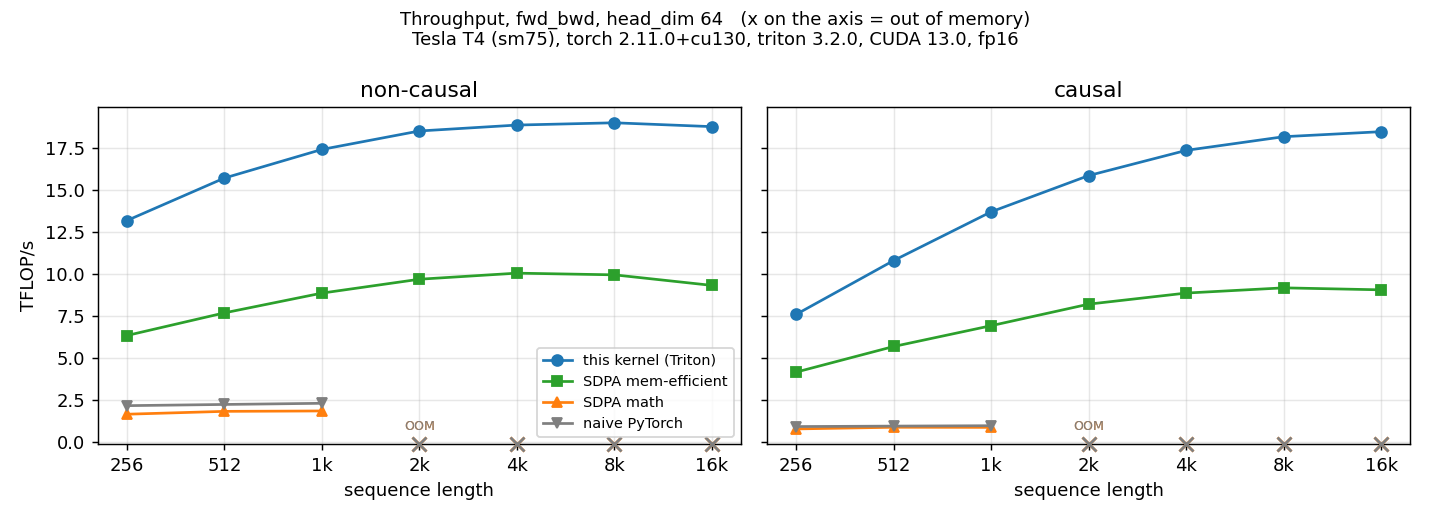
\includegraphics[width=\linewidth]{fig/tflops_fwd_bwd_d64.png}
  \caption{Forward plus backward throughput at head dimension 64 on a Tesla T4
  (fp16, 16k tokens per batch, model width 2048). Left: no mask. Right: causal
  mask. Our kernel (blue) against PyTorch SDPA with the memory-efficient
  backend (green), SDPA with the math backend (orange), and naive PyTorch
  attention (grey). Crosses on the axis mark out-of-memory: naive and math
  attention exceed the T4's 15\,GB from $N=2048$ in this mode.}
  \label{fig:throughput}
\end{figure*}

%%%%%%%%%%%%%%%%%%%%%%%%%%%%%%%%%%%%%%%%%%%%%%%%%%%%%%%%%%%%%%%%%%%%%%%%%%%%%%
\section{Related Work}
\label{sec:related}

\paragraph{Exact attention with less memory.}
Rabe and Staats~\cite{rabe2021selfattention} showed that attention needs only
$O(\sqrt{N})$ or $O(\log N)$ extra memory if the softmax is computed in
chunks. FlashAttention~\cite{dao2022flashattention} turned the same idea into
an IO-aware GPU kernel and proved that it makes asymptotically fewer HBM
accesses than standard attention. FlashAttention-2~\cite{dao2024flashattention2}
parallelizes over query blocks as well as batch and heads, and defers the
softmax normalization to the end of the key loop. FlashAttention-3~\cite{shah2024flashattention3}
targets Hopper with warp specialization, TMA and FP8. PyTorch's
\texttt{scaled\_dot\_product\_attention}~\cite{paszke2019pytorch} dispatches to
a FlashAttention-2 backend on sm80 and newer, and to a memory-efficient
backend derived from xFormers~\cite{lefaudeux2022xformers} on older GPUs. That
memory-efficient backend is our baseline.

\paragraph{Attention variants.}
Multi-query~\cite{shazeer2019fast} and grouped-query
attention~\cite{ainslie2023gqa} share one key/value head among several query
heads to shrink the KV cache. Sliding-window attention~\cite{beltagy2020longformer,
jiang2023mistral} bounds how far back a query may look. Both change which
key tiles a kernel must visit, and both are supported here.

\paragraph{Kernel languages.}
Triton~\cite{tillet2019triton} expresses a kernel as operations on blocks and
leaves thread mapping, shared-memory staging and tensor-core instruction
selection to the compiler. That makes kernels short, but performance then
depends on the compiler release, which \cref{sec:triton} measures.

%%%%%%%%%%%%%%%%%%%%%%%%%%%%%%%%%%%%%%%%%%%%%%%%%%%%%%%%%%%%%%%%%%%%%%%%%%%%%%
\section{FlashAttention-2}
\label{sec:method}

\paragraph{Online softmax.}
For one query row with scores $s_j = \tau\, q \cdot k_j$, $\tau = 1/\sqrt{d}$,
the output is $o = \sum_j e^{s_j - m} v_j / \sum_j e^{s_j - m}$ with
$m = \max_j s_j$. Processing the keys in blocks $B_1, \dots, B_T$, the kernel
keeps a running maximum $m$, a running sum $\ell$ and an unnormalized output
$\tilde{o}$:
\begin{align}
m^{(t)} &= \max\bigl(m^{(t-1)},\, \max_{j \in B_t} s_j\bigr), \nonumber\\
\ell^{(t)} &= e^{m^{(t-1)} - m^{(t)}}\, \ell^{(t-1)} + \textstyle\sum_{j \in B_t} e^{s_j - m^{(t)}}, \label{eq:online}\\
\tilde{o}^{(t)} &= e^{m^{(t-1)} - m^{(t)}}\, \tilde{o}^{(t-1)} + \textstyle\sum_{j \in B_t} e^{s_j - m^{(t)}} v_j, \nonumber
\end{align}
starting from $(-\infty, 0, 0)$. After the last block $o = \tilde{o}^{(T)} /
\ell^{(T)}$ exactly; \cref{sec:proof} gives the induction. FlashAttention-2
divides once at the end, where FlashAttention-1 rescaled $\tilde{o}$ in every
iteration. The kernel saves the log-sum-exp $\mathrm{lse} = m^{(T)} + \log
\ell^{(T)}$ per row, which is the only state the backward pass needs.

\paragraph{Base-2 exponents.}
GPUs evaluate $2^x$ in one instruction. Folding $\log_2 e$ into the scale,
$\hat{s}_j = (\tau \log_2 e)\, q \cdot k_j$, turns every $e^{s - m}$ into
$2^{\hat{s} - \hat{m}}$, and the kernel stores $\lse = \hat{m} + \log_2 \ell$.

\paragraph{Fully masked rows.}
When every score seen so far is masked, $m^{(t)} = -\infty$ and
$m^{(t-1)} - m^{(t)}$ is undefined. The kernel substitutes 0 for $m^{(t)}$ in
the exponent only, so every exponential is $2^{-\infty} = 0$ and the state
stays $(-\infty, 0, 0)$. A row that never sees a key outputs zeros and
$\mathrm{lse} = -\infty$.

\paragraph{Backward pass.}
With $P$ the attention probabilities and $dO$ the output gradient,
\begin{equation}
dV = P^\top dO,\quad dP = dO\,V^\top,\quad dS = P \odot (dP - \delta\mathbf{1}^\top),
\label{eq:bwd}
\end{equation}
then $dQ = \tau\, dS\, K$ and $dK = \tau\, dS^\top Q$, where
$\delta_i = \sum_j P_{ij}\, dP_{ij}$. Because $\sum_j P_{ij} v_j = O_i$,
$\delta_i = dO_i \cdot O_i$, a cheap row-wise reduction (\cref{sec:delta}).
$P$ is never stored: each tile is recomputed as
$P_{ij} = 2^{\hat{s}_{ij} - \lse_i}$.

\paragraph{IO complexity.}
Each query block of $B_r = \Theta(M/d)$ rows reads $K$ and $V$ once, where
$M$ is the on-chip memory per SM. Total HBM traffic is $\Theta(N^2 d^2 / M)$
instead of $\Theta(N^2)$, and extra memory is $\Theta(N)$ for the
log-sum-exp~\cite{dao2022flashattention}. The FLOP count is unchanged.

%%%%%%%%%%%%%%%%%%%%%%%%%%%%%%%%%%%%%%%%%%%%%%%%%%%%%%%%%%%%%%%%%%%%%%%%%%%%%%
\section{Implementation}
\label{sec:impl}

\Cref{fig:kernels} shows the kernels and the data each one reads and writes.
All four are written in Triton with explicit pointer arithmetic and masked
loads, so arbitrary strides and unequal query and key lengths need no copies.
\Cref{tab:compare} compares the design with the reference CUDA implementation.

\begin{figure*}[t]
\centering
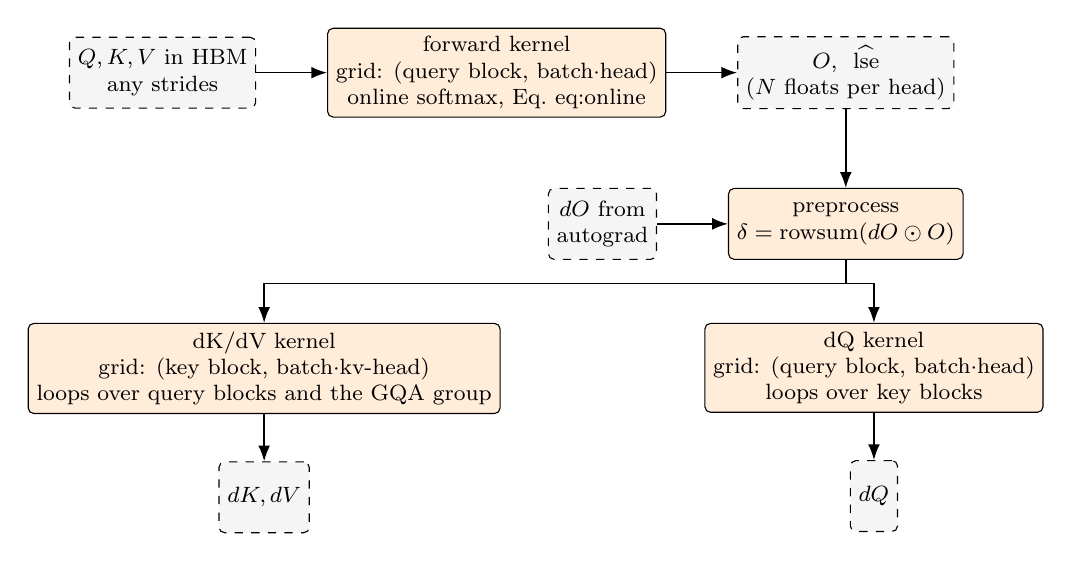
\begin{tikzpicture}[
  node distance=6mm and 9mm,
  box/.style={draw, rounded corners=2pt, align=center, font=\footnotesize, minimum height=9mm, inner sep=3pt},
  hbm/.style={box, dashed, fill=gray!8},
  kern/.style={box, fill=orange!15},
  arr/.style={-{Latex[length=2mm]}, semithick}
]
\node[hbm] (qkv) {$Q, K, V$ in HBM\\ any strides};
\node[kern, right=of qkv] (fwd) {forward kernel\\ grid: (query block, batch$\cdot$head)\\ online softmax, Eq.~\eqref{eq:online}};
\node[hbm, right=of fwd] (olse) {$O$, \ $\lse$\\ ($N$ floats per head)};
\node[kern, below=10mm of olse] (pre) {preprocess\\ $\delta = \mathrm{rowsum}(dO \odot O)$};
\node[hbm, left=of pre] (do) {$dO$ from\\ autograd};
\node[kern, below left=8mm and 6mm of do] (dkdv) {dK/dV kernel\\ grid: (key block, batch$\cdot$kv-head)\\ loops over query blocks and the GQA group};
\node[kern, below right=8mm and 6mm of do] (dq) {dQ kernel\\ grid: (query block, batch$\cdot$head)\\ loops over key blocks};
\node[hbm, below=6mm of dkdv] (dkdvout) {$dK, dV$};
\node[hbm, below=6mm of dq] (dqout) {$dQ$};
\draw[arr] (qkv) -- (fwd);
\draw[arr] (fwd) -- (olse);
\draw[arr] (olse) -- (pre);
\draw[arr] (do) -- (pre);
\draw[arr] (pre.south) |- ++(0,-3mm) -| (dq.north);
\draw[arr] (pre.south) |- ++(0,-3mm) -| (dkdv.north);
\draw[arr] (dkdv) -- (dkdvout);
\draw[arr] (dq) -- (dqout);
\end{tikzpicture}
\caption{Kernels and data flow. Dashed: tensors in global memory; orange:
Triton kernels. The $N \times N$ score and probability matrices exist only as
tiles in registers and shared memory. Both backward kernels recompute
probability tiles from $Q$, $K$ and the saved $\lse$. Each output tile has
exactly one owning program, so no atomics are needed.}
\label{fig:kernels}
\end{figure*}

\begin{table}[t]
\centering
\footnotesize
\setlength{\tabcolsep}{3pt}
\begin{tabular}{@{}p{0.27\linewidth}p{0.32\linewidth}p{0.36\linewidth}@{}}
\toprule
 & FlashAttention-2~\cite{dao2024flashattention2} & This work \\
\midrule
Language & CUDA, CUTLASS & \textbf{Triton, pointer arithmetic} \\
Target & A100, H100 (sm80+) & \textbf{T4 (sm75)} \\
dQ in backward & atomic adds to fp32 buffer & \textbf{separate dQ kernel, deterministic} \\
Matmuls per tile pair (bwd) & 5 & 7 \\
Masks & causal, local window & \textbf{same, one skipping rule} \\
GQA / MQA & yes & yes, \textbf{summed in registers} \\
Variable length & yes & yes \\
Exponent & $e^x$ & $2^x$, scale folded \\
\bottomrule
\end{tabular}
\caption{Design compared with the reference FlashAttention-2 implementation.}
\label{tab:compare}
\end{table}

\subsection{Forward kernel}
One program owns one block of $B_r$ query rows for one (batch, head) pair. It
loads its $Q$ tile once, then streams $K$ and $V$ tiles of $B_c$ keys,
applying \cref{eq:online} with two tensor-core matmuls per tile
(\cref{alg:fwd}). Warps split the query rows of the tile, never the key
columns, so row maxima and sums need no cross-warp exchange. The autotuner
enforces this by rejecting configurations with more than one warp per 16
accumulator rows.

\begin{algorithm}[t]
\caption{Forward kernel, one program}
\label{alg:fwd}
\begin{algorithmic}[1]
\Require query block $b$, head $h$, scale $\hat\tau = \tau \log_2 e$
\State $Q_b \gets$ load rows of block $b$ \Comment{kept in registers}
\State $m \gets -\infty,\ \ell \gets 0,\ \tilde{O} \gets 0$
\State $(lo, f_0, f_1, hi) \gets$ \Call{ScanRange}{$b$, mask}
\For{key tile $j$ in $[lo, hi)$}
  \State $K_j, V_j \gets$ load tile \Comment{masked only at the edges}
  \State $S \gets \hat\tau\, Q_b K_j^\top$
  \If{$j \notin [f_0, f_1)$} $S \gets$ apply mask with $-\infty$ \EndIf
  \State $m' \gets \max(m, \mathrm{rowmax}(S))$
  \State $P \gets 2^{S - m'}$;\ $\alpha \gets 2^{m - m'}$
  \State $\ell \gets \alpha \ell + \mathrm{rowsum}(P)$;\ $\tilde{O} \gets \alpha \tilde{O} + P V_j$
  \State $m \gets m'$
\EndFor
\State store $O_b = \tilde{O} / \ell$ and $\lse_b = m + \log_2 \ell$
\end{algorithmic}
\end{algorithm}

\subsection{Masks and block skipping}
Query $i$ may attend key $j$ when
\begin{equation}
i + \mathrm{off} - L \le j \le i + \mathrm{off} + R, \qquad \mathrm{off} = N_k - N_q,
\label{eq:mask}
\end{equation}
with either bound optional. Causal attention is $R = 0$ without $L$, aligned
to the bottom-right corner as needed when decoding against a longer KV cache.
A finite $L$ is a sliding window. For a block of rows $[r_0, r_1]$, keys
outside $[r_0 + \mathrm{off} - L,\ r_1 + \mathrm{off} + R]$ are invisible to
every row and their tiles are never loaded. Keys inside
$[r_1 + \mathrm{off} - L,\ r_0 + \mathrm{off} + R]$ are visible to every row,
and those tiles run with no mask. Only the edge tiles evaluate the predicate.
The dK/dV kernel solves \cref{eq:mask} for $i$, which is the same form with
$\mathrm{off} \to -\mathrm{off}$ and $L \leftrightarrow R$, so one helper
serves all three kernels. Under a causal mask the forward and dQ kernels
launch the heaviest (last) query blocks first, so the short programs fill the
tail of the launch.

\subsection{Backward kernels}
$dK_j$ and $dV_j$ sum over query rows while $dQ_i$ sums over key columns, so
no single loop order produces all three without accumulating across programs.
The reference implementation adds partial $dQ$ tiles with
atomics~\cite{dao2024flashattention2}. We use two kernels instead. The dK/dV
kernel gives each program a key block and loops over query blocks; the dQ
kernel gives each program a query block and loops over key blocks. Every
output tile has one owner, gradients are bitwise reproducible, and the price
is recomputing $QK^\top$ and $dO\,V^\top$ in both kernels: seven tile matmuls
per (query block, key block) pair instead of five.

\subsection{Grouped-query attention and variable length}
With $H$ query heads and $H_k$ key/value heads, query head $h$ reads
key/value head $\lfloor h / G \rfloor$, $G = H/H_k$. The dK/dV program that
owns a key block loops over the $G$ query heads of its group and sums their
contributions in registers, which needs neither atomics nor a $G$-times larger
buffer. For packed variable-length batches, cumulative offsets give each
program its sequence's start and length. Programs past the end of a shorter
sequence exit immediately.

\subsection{Autotuning}
Block sizes $B_r, B_c \in \{32, 64, 128\}$, 2, 4 or 8 warps and 1 to 3
pipeline stages are searched separately for each kernel, keyed on head
dimension, mask type and a power-of-two length bucket. Before compiling, a
pruner removes configurations whose streamed tiles cannot fit in shared
memory, and multi-stage configurations on GPUs without \texttt{cp.async}
(pre-sm80). The shared-memory estimate is a lower bound, because the real
requirement depends on the compiler release (\cref{sec:triton}). The
autotuner discards configurations the compiler rejects.

%%%%%%%%%%%%%%%%%%%%%%%%%%%%%%%%%%%%%%%%%%%%%%%%%%%%%%%%%%%%%%%%%%%%%%%%%%%%%%
\section{Correctness}
\label{sec:correct}

Every output and gradient is compared with an fp32 reference implementation
of \cref{eq:mask}. Instead of a fixed tolerance, each test measures the error
of PyTorch's own fp16 attention against the same reference and requires
\begin{equation}
\| y - y_{32} \|_\infty \le 2\, \| y_{16} - y_{32} \|_\infty + \epsilon_{\mathrm{dtype}} \cdot s,
\label{eq:tol}
\end{equation}
where $y_{16}$ is the fp16 PyTorch result and $s$ is the largest magnitude
among the reference outputs or gradients. A kernel therefore passes only if
it is about as accurate as the library implementation of the same
computation in the same precision.

The suite covers sequence lengths 1, 17, 200, 1000, 1023, 1024 and 4096;
unequal query and key lengths chosen so that $N_k - N_q \equiv 1$ or
$-2 \pmod{16}$, which places the mask diagonal off every tile boundary;
non-contiguous inputs; every mask type; GQA and MQA; packed batches;
large-logit stability; bitwise determinism; and the autotuner. We checked
the suite by mutation: planting an off-by-one error in the causal mask
originally went undetected, which led to the unequal-length shapes above.

\begin{table}[t]
\centering
\footnotesize
\setlength{\tabcolsep}{4pt}
\begin{tabular}{@{}llrrr@{}}
\toprule
Run & Hardware & Pass & Skip & Fail \\
\midrule
v8 (forward) & T4 & 226 & 90 & 0 \\
v9 (+ backward) & T4 & 403 & 180 & 0 \\
v11 (+ GQA, window) & T4 & 609 & 180 & 0 \\
\textbf{v21 (+ varlen)} & \textbf{T4} & \textbf{629} & \textbf{180} & \textbf{0} \\
local & CPU interp. & 512 & 297 & 0 \\
\bottomrule
\end{tabular}
\caption{Test runs. GPU skips are bf16 cases (the T4 has no bf16 tensor
cores) and GQA cases that duplicate the single-head case. The interpreter
runs small shapes only.}
\label{tab:tests}
\end{table}

%%%%%%%%%%%%%%%%%%%%%%%%%%%%%%%%%%%%%%%%%%%%%%%%%%%%%%%%%%%%%%%%%%%%%%%%%%%%%%
\section{Experimental Setup}
\label{sec:setup}

\paragraph{Hardware and software.}
Kaggle, 2$\times$ Tesla T4 (sm75, 40 SMs, 64\,KB shared memory and 64k
registers per SM, 320\,GB/s, 65\TF{} dense fp16 tensor-core peak), driver
580.178.04, CUDA 13.0, PyTorch 2.11.0, Triton 3.2.0 (\cref{sec:triton}
explains the version), all in fp16.

\paragraph{Workload.}
We follow the FlashAttention-2 benchmark: 16k tokens per batch
(batch $= 16384/N$), model width 2048, hence 32 heads at $d = 64$ and 16 at
$d = 128$; $N$ from 256 to 16,384; with and without a causal mask; forward,
backward, and both.

\paragraph{Baselines.}
Naive attention in PyTorch, and PyTorch SDPA with the backend forced through
\texttt{sdpa\_kernel}: \texttt{MATH} and \texttt{EFFICIENT\_ATTENTION}. SDPA's
FlashAttention backend requires sm80 and is unavailable on the T4.

\paragraph{Measurement.}
\texttt{triton.testing.do\_bench} (25\,ms warm-up, 100\,ms of repetitions,
median), repeated 5 times; we report the median of the medians. One process
per GPU, so no two timed kernels share a device. FLOPs are counted as
$4 B H N^2 d$ for the forward, 2.5$\times$ that for the backward and
3.5$\times$ for both, halved under a causal mask. Clock locking is not
permitted on Kaggle. The median relative spread over the 5 repeats is 0.7\%;
the worst is 28\% for a backward pass that takes under 1\,ms.

%%%%%%%%%%%%%%%%%%%%%%%%%%%%%%%%%%%%%%%%%%%%%%%%%%%%%%%%%%%%%%%%%%%%%%%%%%%%%%
\section{Experiments}
\label{sec:exp}

\subsection{Main result}
\Cref{tab:main} lists the throughput of our kernel and of SDPA
memory-efficient over the sweep. Our forward pass reaches 21 to 25\TF{} at long
sequences, 33\% to 38\% of peak, and forward plus backward 14.6 to 18.8\TF{}.
Across every configuration it is 1.4$\times$ to 2.2$\times$ the baseline. At
$N = 16$k, $d = 64$ without a mask, a forward plus backward pass takes 410\,ms
against 826\,ms.

\begin{table*}[t]
\centering
\footnotesize
\begin{tabular}{@{}lllcccc@{}}
\toprule
Mode & $d$ & Mask & $N=256$ & $N=1$k & $N=4$k & $N=16$k \\
\midrule
\multirow{4}{*}{forward}
 & 64 & none & 19.3 / 10.5 & 22.4 / 11.9 & 22.6 / 12.6 & \textbf{24.5} / 12.6 \\
 & 64 & causal & 12.2 / 8.2 & 16.7 / 11.4 & 22.5 / 12.8 & 24.0 / 13.2 \\
 & 128 & none & 17.8 / 10.0 & 20.9 / 11.6 & 21.8 / 12.0 & 21.4 / 11.8 \\
 & 128 & causal & 10.6 / 7.6 & 17.9 / 10.8 & 21.2 / 12.1 & 22.4 / 11.5 \\
\midrule
\multirow{4}{*}{backward}
 & 64 & none & 12.2 / 5.6 & 15.7 / 7.9 & 17.8 / 9.2 & 17.7 / 8.6 \\
 & 64 & causal & 7.9 / 3.8 & 12.7 / 6.4 & 15.4 / 7.9 & 17.1 / 8.0 \\
 & 128 & none & 8.8 / 6.0 & 13.0 / 8.0 & 13.1 / 8.8 & 13.4 / 8.8 \\
 & 128 & causal & 7.6 / 3.6 & 11.6 / 6.8 & 13.3 / 8.7 & 13.7 / 9.2 \\
\midrule
\multirow{4}{*}{fwd + bwd}
 & 64 & none & 13.2 / 6.3 & 17.4 / 8.9 & 18.9 / 10.0 & \textbf{18.8} / 9.3 \\
 & 64 & causal & 7.6 / 4.1 & 13.7 / 6.9 & 17.4 / 8.9 & 18.5 / 9.1 \\
 & 128 & none & 9.5 / 6.5 & 13.7 / 8.6 & 14.4 / 9.7 & 14.6 / 9.4 \\
 & 128 & causal & 7.5 / 4.2 & 12.3 / 7.9 & 14.7 / 9.8 & 15.0 / 9.9 \\
\bottomrule
\end{tabular}
\caption{Throughput in TFLOP/s on a Tesla T4, ours / SDPA memory-efficient.
The intermediate lengths ($N = 512$, 2k, 8k) were measured as well and are
in the released CSV; they follow the same trend and are omitted for width.}
\label{tab:main}
\end{table*}

\subsection{Analysis}

\paragraph{The backward pass runs the tensor cores as hard as the forward.}
The FLOP convention credits the backward with five $N^2 d$ matmuls; our
atomic-free split executes seven. Scaling the measured 17.7\TF{} ($d = 64$,
$N = 16$k) by $7/5$ gives 24.8\TF{} of executed matmul throughput, the same as
the forward pass at that shape (24.5\TF{}). The 40\% of extra work is the cost
of deterministic gradients.

\paragraph{What limits the T4 to 38\% of peak.}
Three factors are consistent with the measurements. First, sm75 lacks
\texttt{cp.async}, so global loads cannot be software-pipelined and the
autotuner keeps one stage. Second, the forward search picked $B_r{=}128,
B_c{=}64$ in 25 of 28 searches, and the compiled kernels use 128 to 255
registers per thread with no spills. At about 200 registers an 8-warp program
takes roughly 51k of the 64k registers, leaving 8 of 32 warp slots per SM to
hide latency~\cite{volkov2010better}. Third, each $K/V$ tile load feeds
$4 B_r B_c d$ FLOPs for $4 B_c d$ bytes, an intensity of $B_r = 128$
FLOP/byte, below the T4 ridge point of about 200~\cite{williams2009roofline}.
The kernel therefore depends on L2 hits between query blocks of the same head.
Register counts are measured; occupancy and intensity are derived from them,
since hardware counters are not accessible on Kaggle.

\paragraph{Head dimension 128 in the backward.}
The dK/dV kernel holds four $B_c \times d$ tiles ($K$, $V$, $dK$, $dV$) in
registers. At $d = 64$ most dK/dV searches choose $B_c = 128$; at $d = 128$
nearly all fall back to $B_c = 64$, which halves the reuse of every $Q$ and
$dO$ tile loaded. Backward throughput at $d = 128$ stays near 13 to 14\TF{}
against 17 to 18 at $d = 64$.

\paragraph{Short and causal sequences.}
At $N = 256$ a head has two to four query blocks, so the launch has little
parallelism and per-program setup is a large share of the work. Causal
masks add a high fraction of diagonal tiles at short $N$. From $N = 4$k the
causal forward matches the unmasked rate (22.5 against 22.6\TF{} at $d = 64$),
so skipped tiles cost almost nothing.

\paragraph{Memory.}
\Cref{tab:mem} shows peak memory for forward plus backward. Both tiled
kernels are flat in $N$ at a fixed token count, because nothing of size $N^2$
is ever allocated; ours uses 21\% less than the baseline.

\begin{table}[t]
\centering
\footnotesize
\begin{tabular}{@{}lrrrr@{}}
\toprule
Method & $N{=}256$ & $N{=}1$k & $N{=}4$k & $N{=}16$k \\
\midrule
naive PyTorch & 1794 & 5634 & OOM & OOM \\
SDPA math & 2944 & 9088 & OOM & OOM \\
SDPA mem.-efficient & 900 & 900 & 900 & 900 \\
\textbf{ours} & \textbf{708} & \textbf{708} & \textbf{708} & \textbf{708} \\
\bottomrule
\end{tabular}
\caption{Peak GPU memory in MB for forward plus backward, $d = 64$, no mask,
16k tokens at every $N$.}
\label{tab:mem}
\end{table}

\subsection{Compiler version on Turing}
\label{sec:triton}

The first full benchmark run used the Triton release bundled with the
platform, 3.6.0. All correctness tests passed, but the forward pass measured
1.2\TF{} and the backward 0.5\TF{}, 10$\times$ to 50$\times$ below
\cref{tab:main}. We compiled the kernels and read the generated PTX: there
were no tensor-core \texttt{mma} instructions and up to 1,870 spilled registers
per kernel. A ten-line Triton matmul behaved the same way (1.2\TF{} against
18\TF{} for \texttt{torch.mm} on the same GPU), which ruled out the attention
code. Keeping the source fixed and changing only the Triton release isolated
the regression (\cref{tab:triton}).

\begin{table}[t]
\centering
\footnotesize
\setlength{\tabcolsep}{4pt}
\begin{tabular}{@{}lccl@{}}
\toprule
Triton & matmul & ours, fwd & code for \texttt{tl.dot} \\
\midrule
\textbf{3.2.0} & \textbf{21.4} & \textbf{17.2} & \texttt{mma.sync}, no spills \\
3.3.1 & \multicolumn{2}{c}{compile error} & fp16 conversion fails \\
3.4.0 & 1.2 & 1.22 & scalar \texttt{fma} \\
3.5.1 & 1.3 & 1.14 & scalar \texttt{fma} \\
3.6.0 & 1.2 & 1.25 & scalar \texttt{fma}, spills \\
\bottomrule
\end{tabular}
\caption{Triton release against throughput (TFLOP/s) on a T4: the best of
three tile sizes for a 2048$^3$ fp16 matmul, and our forward pass at $d=64$,
$N=1$k with fixed blocks. Releases before 3.2 have no wheels for the Python
version on the platform.}
\label{tab:triton}
\end{table}

The repository therefore installs Triton 3.2.0 on pre-sm80 GPUs and warns at
runtime when an affected release runs on sm7x. The same comparison showed that
the shared-memory requirement of a configuration depends on the release: the
$B_r{=}128$, $B_c{=}64$, $d{=}128$ forward tile needs 98\,KB under 3.6 and fits
in 64\,KB under 3.2, where it is the fastest $d = 128$ configuration. This is
why the pruner's estimate is a lower bound.

\subsection{End-to-end training}
\label{sec:train}

We trained a character-level GPT on TinyShakespeare~\cite{karpathy2015charrnn}
twice, changing only the attention function (\cref{tab:train}): 6 layers,
width 512, 8 heads, context 1024, 19.4M parameters, batch 8 per GPU, DDP on
both T4s, fp16 autocast with a gradient scaler, AdamW ($\beta = (0.9, 0.95)$,
weight decay 0.1), learning rate $10^{-3}$ with 100 warm-up steps and cosine
decay to $10^{-4}$, gradient clipping at 1.0, 2000 steps, seed 1234.

\begin{table}[t]
\centering
\footnotesize
\setlength{\tabcolsep}{4pt}
\begin{tabular}{@{}lrrrr@{}}
\toprule
Attention & tokens/s & MB/GPU & best val & final val \\
\midrule
\textbf{ours} & \textbf{161,477} & 1392 & \textbf{1.526} & \textbf{2.008} \\
SDPA mem.-efficient & 152,861 & 1346 & 1.531 & 2.123 \\
\bottomrule
\end{tabular}
\caption{GPT training on 2$\times$ T4. ``Best val'' is the validation loss at
step 1000, the minimum for both runs.}
\label{tab:train}
\end{table}

\begin{figure}[t]
  \centering
  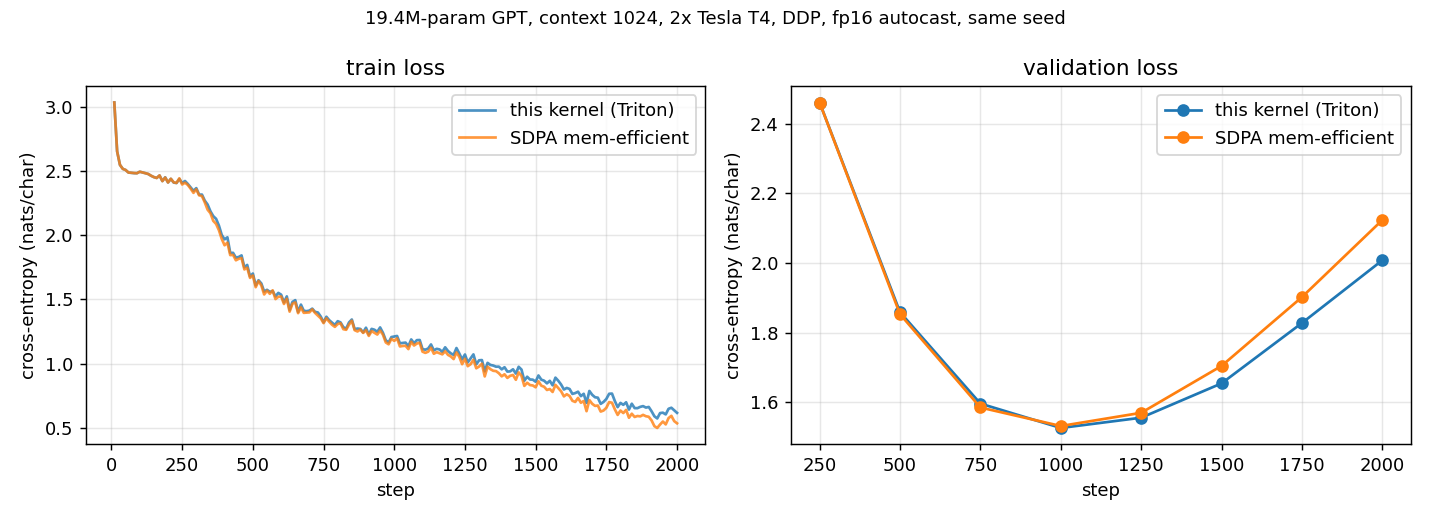
\includegraphics[width=\linewidth]{fig/loss_curves.png}
  \caption{Training and validation loss with our kernel and with SDPA
  memory-efficient attention, same seed and data order. Both models overfit
  after step 1000.}
  \label{fig:loss}
\end{figure}

End-to-end training is 5.6\% faster. The gain is far below the kernel
speedup because at this size attention is a minority of each step: the MLPs,
the vocabulary projection, the optimizer and the gradient all-reduce take the
rest. The loss curves (\cref{fig:loss}) overlap until both models begin to
overfit. To judge the later gap we compared two SDPA runs with identical code
and seed. They differ by 0.018 on average and 0.052 at most in training loss,
and end at validation losses 2.048 and 2.123. Our kernel differs from SDPA by
0.031 on average and 0.089 at most, the same order as the baseline's own
run-to-run variation from fp16 rounding and non-deterministic reductions
compounding over 2000 steps.

%%%%%%%%%%%%%%%%%%%%%%%%%%%%%%%%%%%%%%%%%%%%%%%%%%%%%%%%%%%%%%%%%%%%%%%%%%%%%%
\section{Computational Efficiency}
\label{sec:efficiency}

At $N = 16$k and $d = 64$ the model of \cref{sec:setup} spends 410\,ms on
attention forward and backward with our kernel, 826\,ms with SDPA
memory-efficient attention, and runs out of memory with naive or math
attention. Our kernel's peak memory of 708\,MB is flat in $N$, so on a 15\,GB
T4 the sequence length is limited by the activations of the rest of the model
rather than by attention. A full benchmark sweep, the GPU test suite and the
training demo run in 51 minutes on one Kaggle session.

%%%%%%%%%%%%%%%%%%%%%%%%%%%%%%%%%%%%%%%%%%%%%%%%%%%%%%%%%%%%%%%%%%%%%%%%%%%%%%
\section{Limitations}
\label{sec:limits}

All performance results come from one GPU model. On Ampere, \texttt{cp.async}
would make multi-stage pipelining useful and larger shared memory would admit
larger tiles; on Hopper, the explicit pointer arithmetic leaves TMA and warp
specialization unused, which is where FlashAttention-3 gains most. Neither was
measured. bf16 is implemented but has not run on hardware, because the T4 has
no bf16 tensor cores. GPU clocks could not be locked. The variable-length grid
is sized for the longest sequence, so programs beyond a shorter sequence are
launched and exit at once. Dropout, attention bias and a KV-cache decoding
path are not implemented.

%%%%%%%%%%%%%%%%%%%%%%%%%%%%%%%%%%%%%%%%%%%%%%%%%%%%%%%%%%%%%%%%%%%%%%%%%%%%%%
\section{Conclusion}
\label{sec:conclusion}

We implemented FlashAttention-2 from scratch in Triton, with masking,
grouped-query attention and variable-length batches, and an atomic-free
backward pass that is deterministic and, corrected for recomputation, as
efficient as the forward. On a Tesla T4 it reaches 24.5\TF{} forward and
18.8\TF{} forward plus backward, 1.4$\times$ to 2.2$\times$ PyTorch's
memory-efficient attention, uses 21\% less memory, and trains a GPT 5.6\%
faster with loss curves within the baseline's own run-to-run variation. The
largest single effect on performance was not in the kernel at all: on Turing
GPUs, the Triton release decides whether \texttt{tl.dot} uses tensor cores.
Reading the generated code, rather than tuning the kernel, found it.

\paragraph{Declaration of resources.}
Kernels are written in Triton 3.2.0 and the surrounding code in PyTorch
2.11.0, with NumPy and Matplotlib for analysis. All GPU runs used Kaggle's
free 2$\times$ Tesla T4 environment; local development used the Triton CPU
interpreter. No pretrained model is used. Code, raw benchmark data and the
output of every GPU run are available at
\url{https://github.com/AAK121/flash-attention-triton}.

{
    \small
    \bibliographystyle{ieeenat_fullname}
    \bibliography{main}
}

%%%%%%%%%%%%%%%%%%%%%%%%%%%%%%%%%%%%%%%%%%%%%%%%%%%%%%%%%%%%%%%%%%%%%%%%%%%%%%
\clearpage
\setcounter{page}{1}
\maketitlesupplementary
\appendix

\section{Correctness of the online softmax}
\label{sec:proof}

\textbf{Claim.} After block $t$ of \cref{eq:online},
$\ell^{(t)} = \sum_{j \in B_{\le t}} e^{s_j - m^{(t)}}$ and
$\tilde{o}^{(t)} = \sum_{j \in B_{\le t}} e^{s_j - m^{(t)}} v_j$.

\textit{Proof by induction.} For $t = 1$ the correction factor multiplies the
zero initial state. Assume the claim for $t-1$. Since
$e^{s_j - m^{(t-1)}}\, e^{m^{(t-1)} - m^{(t)}} = e^{s_j - m^{(t)}}$,
\[
e^{m^{(t-1)} - m^{(t)}}\, \ell^{(t-1)} = \sum_{j \in B_{<t}} e^{s_j - m^{(t)}},
\]
and adding the block-$t$ terms gives the sum over $B_{\le t}$. The same algebra
holds for $\tilde{o}$. Hence $\tilde{o}^{(T)} / \ell^{(T)}$ equals the softmax
output exactly: the recurrence reassociates the same sums. Every exponent is
at most 0 because $m^{(t)}$ bounds all scores seen, so no term overflows.
$\square$

\section{Derivation of $\delta$}
\label{sec:delta}

The row-wise softmax $p = \mathrm{softmax}(s)$ has Jacobian
$\mathrm{diag}(p) - p p^\top$, so
$dS_i = p_i \odot dP_i - p_i\, (p_i^\top dP_i) = p_i \odot (dP_i - \delta_i)$
with $\delta_i = p_i^\top dP_i$. Computing it directly needs a full row of
$P$ and $dP$. Instead,
\[
\delta_i = \sum_j P_{ij} (dO_i \cdot v_j)
= dO_i \cdot \Bigl(\sum_j P_{ij} v_j\Bigr) = dO_i \cdot O_i,
\]
an $O(Nd)$ reduction over tensors that already exist. The preprocessing
kernel in \cref{fig:kernels} computes it once before both backward kernels.

\section{Block-skipping work}
\label{sec:skip}

Under a causal mask with $N_q = N_k = N$ and square tiles of size $b$, the
number of tile pairs a program visits sums to
$\sum_{i=1}^{N/b} i = \tfrac{1}{2}(N/b)(N/b + 1)$, about half the unmasked
count. The diagonal adds the $(N/b)/2$ excess, which is why causal
throughput trails the unmasked rate at short $N$ and catches up at long $N$
(\cref{tab:main}). For a window of width $W = L + R + 1$ the visited pairs are
$O\bigl((N/b)(W/b + 2)\bigr)$, linear in $N$.

\section{Autotuner choices}
\label{sec:tune}

From the autotuning logs of the final benchmark run (28 searches per
kernel): the forward kernel chose $B_r{=}128$, $B_c{=}64$ in 25 searches (13
with 8 warps, 12 with 4). The dK/dV kernel chose $B_c{=}128$ keys per program
at $d = 64$ in most searches and $B_c{=}64$ at $d = 128$ in nearly all. The dQ
kernel chose $64 \times 64$ tiles with 4 warps in 17 searches. Multi-stage
configurations never reach the search on the T4: the pruner removes them
because sm75 has no
\texttt{cp.async}.

\end{document}
